\documentclass[fleqn]{template}
\usepackage[english]{babel}
\usepackage{underscore}

% packages andrea used, prob. delete
%\usepackage{float}                                                              
%\usepackage{booktabs}                                                           
%\usepackage{footnotes}                                                          
%\usepackage{graphicx}  

\usepackage{pifont}
\setlength{\columnsep}{0.55cm}
% Distance between the two columns of text
\setlength{\fboxrule}{0.75pt}
% Width of the border around the abstract
\definecolor{color1}{RGB}{88,116,143}
\definecolor{color2}{RGB}{0,20,20} 


\usepackage{hyperref} % Required for hyperlinks
\hypersetup{hidelinks,colorlinks,breaklinks=true,urlcolor=color2,citecolor=color1,linkcolor=color1,bookmarksopen=false,pdftitle={Title},pdfauthor={Author}}


\usepackage{tikz}
\usepackage{verbatim}
%\usepackage[active,tightpage]{preview}
%\PreviewEnvironment{tikzpicture}
%\setlength\PreviewBorder{10pt}%
\usetikzlibrary{arrows,shapes,positioning,shadows,trees}

\usepackage{listings}
%% json style
\lstset{
    string=[s]{"}{"},
    stringstyle=\color{color1},
    comment=[l]{:},
    breaklines=true,
    commentstyle=\color{color2},
}

\usepackage{balance}

\usepackage{subfig}
\usepackage[font=bf,skip=\baselineskip]{caption}


\newcommand{\sd}[1]{\textbf{\color{olive}/* #1 (sd) */}}
\newcommand{\dd}[1]{\textbf{\color{red}/* #1 (dd) */}}
\newcommand{\wo}[1]{\textbf{\color{orange}/* #1 (wo) */}}
\newcommand{\kb}[1]{\textbf{\color{blue}/* #1 (kb) */}}
\newcommand{\az}[1]{\textbf{\color{blue}/* #1 (az) */}}



\begin{document}
    \JournalInfo{GESIS} 

% Additional notes (e.g. copyright, DOI, review/research article)
\Archive{Book Chapter for RCC Book (Sage)}
\PaperTitle{Rich Context Competition Phase 2 (RCC-05)}

\Authors{Wolfgang Otto\textsuperscript{1}*,
         Andrea Zielinski\textsuperscript{1},
         Behnam Ghavimi\textsuperscript{1},
         Dimitar Dimitrov\textsuperscript{1},
         Narges~Tavakolpoursaleh\textsuperscript{1}
        }

\affiliation{\textsuperscript{1}\textit{Email: firstname.lastname@gesis.org. Affiliation: Knowledge Technologies in the Social Sciences, GESIS -- Leibniz Institute for the Social Sciences, Cologne, Germany}} % Author affiliation

\affiliation{*\textbf{Corresponding author}: wolfgang.otto@gesis.org} % Corresponding author

% Keywords - if you don't want any simply remove all the text between the curly brackets
\Keywords{Dataset Mention Extraction --- Dataset Linking --- Research Method Extraction ---  Research Field Classification} 
 % Defines the keywords heading name
\newcommand{\keywordname}{Keywords}

\Abstract{This document describes the approach, results, and software submitted by team RCC-05 to the Rich Context Competition (RCC).
The team consists of members of the department \emph{Knowledge Technologies in the Social Sciences} of \emph{GESIS - Leibniz Institute for the Social Sciences} The goal of the RCC is to automatically discover and link research datasets, methods, and fields in social science publications. 
%The team was selected as one of four out of 19 participants in the first Phase of the competition to attend to the second Phase.
%This document describe the result of the work for both phases.
}

% create front
\flushbottom % Makes all text pages the same height
\maketitle % Print the title and abstract box
\thispagestyle{empty} % Removes page numbering from the first page

 % Front is not shown in markdown
    \section{GESIS}
    \emph{Wolfgang Otto, Andrea Zielinski, Behnam Ghavimi, Dimitar Dimitrov, Narges~Tavakolpoursaleh}
    % \subsection{Abstract}
    % abstract if needed
    
    
    \subsection {Introduction}
%\addcontentsline{toc}{section}{Introduction}

% GESIS & mission
% WTS & mission
% information extraction at WTS
% RCC
% stage 1 feedback 
% stage 2 approach and results
% remaining chapter

GESIS - the Leibniz Institute for the Social Sciences (GESIS)\footnote{\url{https://www.gesis.org/en/institute}} is the largest European research and infrastructure provider for the social sciences and offers research data, services and infrastructures supporting all stages of the scientific process. The GESIS department \textit{Knowledge Technologies for the Social Sciences (WTS)}\footnote{\url{ https://www.gesis.org/en/institute/departments/knowledge-technologies-for-the-social-sciences/}} is responsible for developing all digital services and research data infrastructures at GESIS and aims at providing integrated access to social sciences data and services. Next to traditional social sciences research data, such as surveys and census data, an emerging focus is to build data infrastructures able to exploit novel forms of social sciences research data, such as large Web crawls and archives. 

Research at WTS\footnote{\url{https://www.gesis.org/en/research/applied-computer-science/labs/wts-research-labs}} addresses areas such as Information Retrieval~(IR), Information Extraction~(IE) {\&} Natural Language Processing~(NLP), semantic technologies and human computer interaction and aims at ensuring access and use of social sciences research data along the FAIR principles, for instance, through interlinking of research data, established vocabularies and knowledge graphs and by facilitating semantic search across distinct platforms and datasets. Due to the increasing importance of Web- and W3C standards as well as Web-based research data platforms, in addition to traditional research data portals, findability and interoperability of research data across the Web constitutes one current challenge. In the context of Web-scale reuse of social sciences resources, the extraction of structured data about scholarly entities such as datasets and methods from unstructured and semi-structured text, as found in scientific publications or resource metadata, is crucial in order to be able to uniquely identify social sciences resources and to understand their inherent relations. 

% prior work: scientifically (disambiguation, extraction, publications, web) etc tools (GESIS datasearch, GWS etc)
Prior works at WTS/GESIS addressing such challenges apply NLP and machine learning techniques to, for instance, extract and disambiguate mentions of datasets\footnote{\url{https://www.gesis.org/en/research/external-funding-projects/archive/infolis-i-and-ii}} \cite{boland2012identifying,ghavimi2016semi}), authors \cite{conf/cikm/Backes18, conf/jcdl/Backes18} or software tools \cite{boland2019distant} from scientific publications or to extract and fuse scholarly data from large-scale Web crawls \cite{journals/semweb/YuGFLRD19, sahoo2015analysing}. Resulting pipelines and data are used to empower scholarly search engines such as the \textit{GESIS-wide search}\footnote{\url{https://search.gesis.org}}  \cite{conf/jcdl/HienertKBZM19} which provides federated search for scholarly resources (datasets, publications etc.) across a range of GESIS information systems or the \textit{GESIS DataSearch} platform\footnote{\url{https://datasearch.gesis.org/}} \cite{Krmer2018ADD}, which enables search across a vast number of social sciences research datasets mined from the Web. 
%TODO other papers worth citing here?

% RCC
Given the strong overlap of our research and development profile with the recent initiatives of the Coleridge Initiative to evolve this research field through the Rich Context Competition (RCC)\footnote{\url{https://coleridgeinitiative.org/richcontextcompetition}}, we are enthusiastic about having participated in the RCC2018 and are looking forward to continue this collaboration towards providing sound frameworks and tools which automate the process of interlinking and retrieving scientific resources.

The central tasks in the RCC are the extraction and disambiguation of mentions of datasets and research methods as well as the classification of scholarly articles into a discrete set of research fields. After the first phase, each team received feedback from the organizers of the RCC consisting of a quantitative and qualitative evaluation. Whereas quantitative results of our inital contribution throughout phase one have shown significant room for improvement, the qualitative assessement, conducted by four judges on a sample of ten documents, underlined the potential of our approach. 

%Judges are then asked to manually extract dataset mentions and calculate the overlap between their dataset extractions and the output of our algorithm.
%Other factors that judges took into consideration are specificity, uniqueness, and multiple occurrences of dataset mentions.
%As for the extraction of research methods and fields, no ground truth has been provided; these tasks were evaluated against the judges' expert knowledge.
%Similarly to the extraction of dataset mentions, specificity and uniqueness have been considered for these two tasks.

Since we have been shortlisted for the second phase of the RCC, this chapter describes our approaches, techniques, and additional data used to address all three tasks. As described in the following subsections, we decided to follow a module-based approach where each module or the entire pipeline can be reused. The remaining chapter is organised as follows.
The following Section~\ref{sec:overview} provides an overview of our approach, used background data and preprocessing steps, whereas Sections ~\ref{sec:dataset-extraction}, ~\ref{sec:research_method_extraction} and ~\ref{sec:field_classification} describes our approaches in more detail, including results towards each of the tasks. Finally, we discuss our results in Section~\ref{sec:discussion} and provide an overview of future work in Section~\ref{sec:conclusion}.
%TODO best to add a short conclusion/future work section.




    \subsection{Approach, data and pre-processing}
\label{sec:overview}
This section describes the external data sources we used as well as our pre-processing steps.

%\subsubsection{The RCC Corpus}
%\label{subsec:rcc-corpus}
%For the first phase, the data provided by the organizers consisted of 5,000 publications. Additionally, a development fold of 100 plain text publications, their metadata, a list of datasets of interest (including all datasets that were explicitly referenced in the curated corpus) were given. The list of datasets should not be considered complete as  there could be additional datasets mentioned in these publications. 
%The organizers also provided examples of social science research methods and fields vocabularies in term of SAGE Publications research field and method vocabularies. 
%In the second phase of the competition, an additional set of 5,000 publications from the social sciences has been provided.

%TODO include subsubsection on "Approach overview and initial evaluation feedback" where we can include the overview of the modules and more details on the first stage evaluation (I've been cutting these parts a lot in the introduction to keep it more general)

\subsubsection{Approach overview and initial evaluation feedback}
\label{sec:approach_feedback}




%\subsection{Task Definition of the RCC}
%In both competition phases the task was to submit a software package which is able to process PDF (respectively extracted raw text) on the Servers of the organizers.
%The software have to be able to extract dataset mentions, research methods and research fields from the given publication. More about the type of scientific publications can be found in Section~\ref{subsec:rcc-corpus}.
%In the first phase additional the software has to be able to link dataset mentions to a given set of around 10,000 dataset descriptions originate from ICPSR\footnote{\url{https://www.icpsr.umich.edu/icpsrweb/ICPSR/}} research data index.


%\subsubsection{Non-technical overview}

%\begin{itemize}
%    \item Usage of external data
%    \item Supervised machine learning Approaches
%    \item Problem of Training data: weak supervision
%\end{itemize}


% Literature Review


The central tasks in the RCC are the extraction of dataset mentions from text. 
Even so, we considered the discovery of research methods and research fields important.
To this end, we decided to follow a module-based approach. Users could choose to use each specific module solely or as parts of a data processing pipeline.
Figure~\ref{figure:pipeline} shows an overview of modules developed and their dependencies.
Here, the upper three modules (which are in gray) describe the pre-processing steps (cf. Section~\ref{sec:prepro}).
The lower four modules (blue) are used to generate the output in a predefined format as specified by the competition.


\begin{figure}[t]
    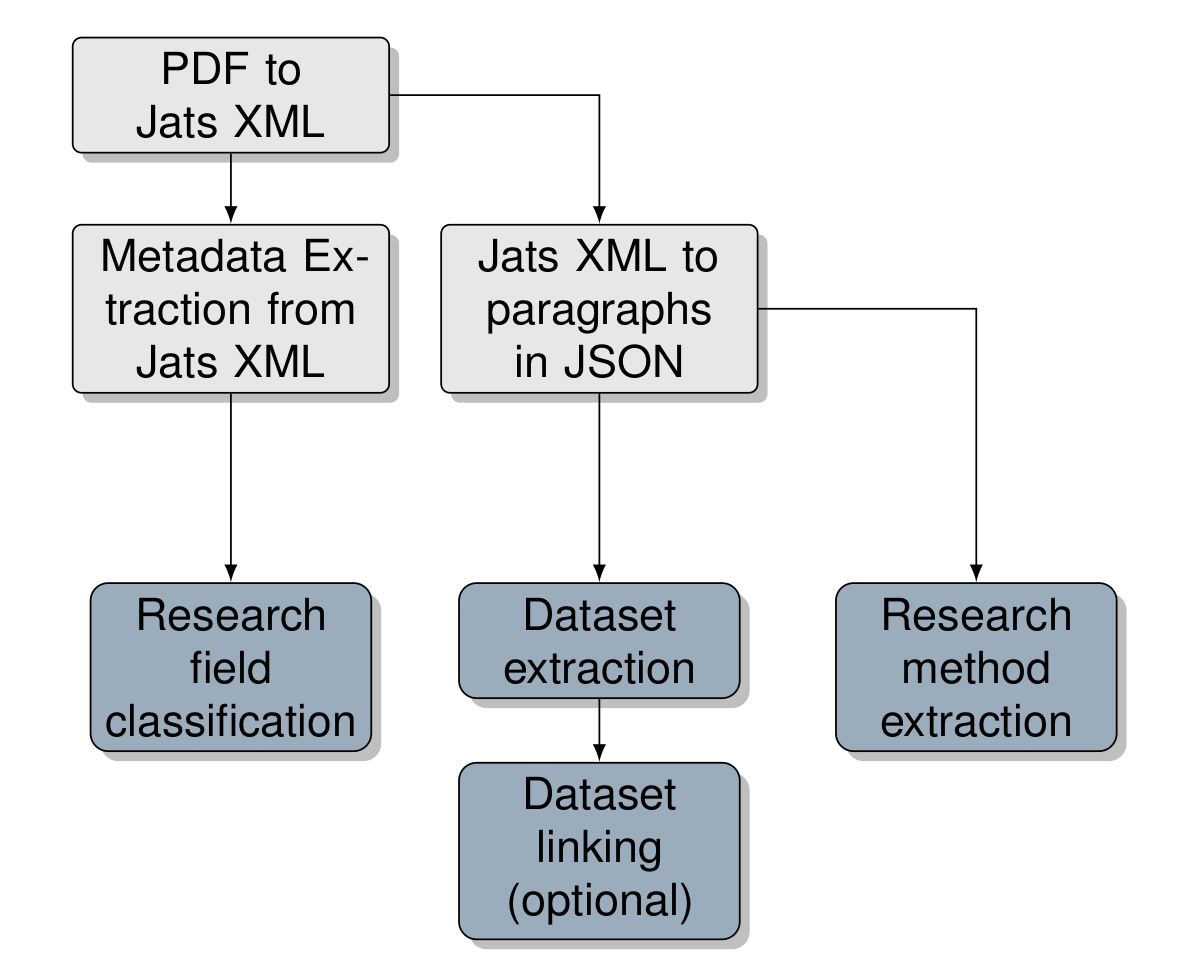
\includegraphics[width=0.47\textwidth]{figures/information-flow.png}
    %% Graphic from tex
    %\resizebox{!}{7cm}{\tikzset{
  basic/.style  = {draw, text width=2cm, drop shadow, font=\sffamily, rectangle},
  root/.style   = {basic, rounded corners=2pt, thin, align=center,
                   fill=color1!30},
  level empty/.style={},
  level 1/.style={sibling distance=2mm},
  level 2/.style = {basic, rounded corners=4pt, thin, align=center, fill=color1!60},
  level 3/.style = {basic, rounded corners=2pt, thin,
                    align=center, fill=color2!10, text width=6.5em}
}


\begin{tikzpicture}[
  node distance=1.7cm and 1.7cm,
  edge from parent/.style={->,draw},
  >=latex
  ]

% root of the the initial tree, level 1
%\node[root] {RCC-05 Pipeline Components}
% The first level, as children of the initial tree
%  child {node[level 2] (c1) {Preprocessing}}
%  child {node[level 2] (c2) {Dataset Linking}}
%  child {node[level 2] (c3) {Research Method Extraction}}
%  child {node[level 2] (c4) {Research Field Classification}};

% The second level, relatively positioned nodes
\begin{scope}[every node/.style={level 3}]
    \node [] (c11) {PDF to Jats XML};
    \node [below of = c11] (c12) {Metadata Extraction from Jats XML};
    \node [right = 0.4cm of c12] (c13) {Jats XML to paragraphs in JSON};
\end{scope}

\node [level 2, below = 1.5cm of c13, xshift=0pt] (c21) {Dataset extraction};
\node [level 2, below =  0.5cm of c21] (c22) {Dataset linking (optional)};
\node [level 2, below = 1.5cm of c13, xshift=3cm]  (c31) {Research method extraction};
\node [level 2, below = 1.5cm of c12, xshift=0pt] (c41) {Research field classification};

\node [level empty, below = 2.7cm of c21] (c51){};
 



% lines from each level 1 node to every one of its "children"
%\foreach \value in {1,...,3}
%  \draw[->] (c1.195) |- (c1\value.west);
%\draw[->] (c1.south) -| (c11.north);
\draw[->] (c11.south) -| (c12.north);
\draw[->] (c11.east)  -- +(1,0) -| (c13.north);

\draw[->] (c13.south) -| (c21.north);
\draw[->] (c21.south) -| (c22.north);

\draw[->] (c13.east) -- +(1.7,0) -| (c31.north);

\draw[->] (c12.south) -| (c41.north);

%\foreach \value in {1,...,1}
%  \draw[->] (c3.195) |- (c3\value.west);
\end{tikzpicture}

\begin{comment}
    Old Pipeline (4 Elements)
    \node[level 2] (c1) {(1) Preprocessing};
    \node[level 2, right= 3cm of c1] (c2) {(2) Dataset Linking};
    \node[level 2, right= of c2] (c3) {(3) Research Method Extraction};
    \node[level 2, right= of c3] (c4) {(4) Research Field Classification};
    \draw[->] (c1) |- (c2);
    \draw[->] (c1.30) -- +(0,0.7) -| (c3.north);
    \draw[->] (c1.150) -- +(0,1.3) -| (c4.north);

\end{comment}
}
    \caption{An overview of the individual software modules described in this document and their dependencies. 1- Gray: Our pre-processing pipeline. 2- Blue: three main tasks of the RCC.}
    \label{figure:pipeline}
\end{figure}

%TODO I'd suggest to use the same wording in the figure as in the following section headings, e.g. "Resarch field classification" etc. Also, I would not use color-coding (always ambiguous on b/w printing).

The pre-processing step consists of extracting metadata and raw text from PDF documents.
The output of this step is then used by the software modules responsible for tackling the individual sub-tasks.
These sub-tasks are to discover research datasets (cf. Section~\ref{sec:dataset-extraction}), methods (cf. Section~\ref{sec:research_method_extraction}) and fields (cf. Section~\ref{sec:field_classification}).
First, a Named Enity Recognition module is used to find dataset mentions.
This module used a supervised approach trained on a weakly labled corpus.
%The creation of the used training corpus and the model are described in Section~\ref{sec:dataset-extraction}.
In the next step, we combine all recognized mentions for each publication and compare these mentions to the metadata from the list of datasets given by the competition. %`data_sets.json`.
For this linking step the mentions and year information located in the same sentence are used.
The corresponding sentence and extracted information are saved for debugging and potential usage in future pipeline components.
%After retrieving the best matching results, theses are returned in the target format specified by the RCC-competition.
The task of identifying research methods is done by an adjusted NER module trained on a corpus of scientific publications. 
For identifying research fields, we trained a classifier on openly available abstracts and metadata from the domain of social sciences crawled from the Social Science Open Access Repository\footnote{\url{https://www.ssoar.info}} (SSOAR).
%We used the OAI-API for this and the crawler is delivered in the module.
We tried different classifiers and selected the best performing one, a classifier based on fasttext\footnote{\url{https://fasttext.cc/}}, i.e. a neural net based approach with a high performance\cite{joulin2017bag}.



After the first phase, each team received feedback from the organizers of the RCC.
The feedback is two folds, a quantitative and qualitative evaluation. Unfortunately, the quantitative assessment showed our algorithms did not perform well regarding precision and recall metrics. In contrast to this, our approach has been found convincing regarding the quality of results. The qualitative feedback was from a random sample of ten documents given to four judges.
Judges are then asked to manually extract dataset mentions and calculate the overlap between their dataset extractions and the output of our algorithm.
Other factors that judges took into consideration are specificity, uniqueness, and multiple occurrences of dataset mentions.
As for the extraction of research methods and fields, no ground truth has been provided; these tasks were evaluated against the judges' expert knowledge.
Similarly to the extraction of dataset mentions, specificity and uniqueness have been considered for these two tasks.
The feedback our team received acknowledged the fact that no ground truth has been provided and our efforts regarding the extraction of research methods and fields.
%Feedback by RCC
%Section~\ref{} gives detailed overview of data provided by the RCC and additional data sources used in our approach. :o .

\subsubsection{External data sources}
\label{sec:external_data_sources}
For developing our algorithms, we utilized two external data sources.
For the discovery of research methods and fields, we resort to data from the Social Science Open Access Repository\footnote{\url{https://www.gesis.org/ssoar/home}} (SSOAR). 
GESIS – Leibniz Institute for the Social Sciences maintains  SSOAR by collecting and archiving literature of relevance to the social sciences. 

In SSOAR, full texts are indexed using controlled social science vocabulary (Thesaurus\footnote{\url{https://www.gesis.org/en/services/research/tools/thesaurus-for-the-social-sciences}}, Classification\footnote{\url{https://www.gesis.org/angebot/recherchieren/tools-zur-recherche/klassifikation-sozialwissenschaften} (in German)}) and are assigned rich metadata. SSOAR offers documents in various languages. The corpus of English language publications that can be used for purposes of the competition consists of a total of 13,175 documents. All SSOAR documents can be accessed through the OAI-PMH\footnote{{\url{http://www.openarchives.org}}} interface. 

Another external sourcei, that we used for the discovery of research methods is the ACL Anthology Reference Corpus~\cite{bird2008acl}. ACL ARC is a corpus of scholarly publications about computational linguistics.  
The corpus consists of a total of 22,878 articles.

%SSOAR contains 
%\subsubsection{SSOAR}
%\label{subsubsec:ssoar-dataset}
%For example, 22,453 records with English abstracts in SSOAR also contain information about the classification of social sciences documents - 156 different labels of the classification.
%For items with English title and classoz classification, the numbers are different. SSOAR includes 15,522 items with English titles and cover 154 classoz classification labels.
%Classification Schemes used in the anntotations of SSOAR publications.
%\begin{enumerate}
%    \item Thesaurus Social Science (thesoz)
%    \item classification of the social sciences %(classoz)\footnote{\url{https://www.gesis.org/angebot/recherchieren/tools-zur-recherche/klassifikation-sozialwissenschaften} (in German)}
%    \item ddc classification (ddc)
%\end{enumerate}

%\subsubsection{ACL}
%ACL 

%\dd{table of external data/sources?SSOAR metedata including abstracts and classifications(thesoz/ classsoz)}

\subsubsection{Pre-processing}
\label{sec:prepro}
Although the organizers of the RCC offered plain texts for the publication, we decided to build our own pre-processing pipeline.
The extraction of text from PDF files is still an error prone process. To handle de-hyphenation and paragraph segmentation during extraction time and benefit from automatic metadata extraction (i.e. title, author, abstracts and references) we decided to use a third party extraction tool.
The Cermine Extraction Tool\footnote{\url{https://github.com/CeON/CERMINE}}\cite{tkaczyk2015cermine} transforms the files into XML documents using the Journal Article Tag Suite\footnote{\url{https://jats.nlm.nih.gov}}(Jats).
%The main benefit of using this tool is the structured metadata output, including better disambiguation of sections and paragraphs in the publications.
For the competition we identified two interesting elements of the Jats XML format, i.e., $<$front$>$ and $<$body$>$. The $<$front$>$ element contains the metadata of the publication, whereas the $<$body$>$ contains the main textual and graphic content of the publication.
%A benefit of Cermine is that the de-hyphenation and segmentation of paragraphs are carried out out of the box.
As a last step of the pre-processing, we removed all linebreaks from the publication.
The output of this step is a list of metadata fields and values, as shown in Table~\ref{tab:example-paragraph} for each publication paragraph.

\begin{table}[h]
    \centering
     \caption{Example preprocessing output for a paragraph in a given publication.}
    \begin{tabular}{ll}
        \toprule
        {}                  &                            Example Text Field Data \\
        \midrule
        publication\_id     &                                              12744 \\
        label               &                                    paragraph\_text \\
        text                &                     A careful reading of text, word\\
                            &                                  for word, was ... \\
        section\_title      &                                      Data Analysis \\
        annotations         &                        [\{'start': 270, 'end': 295,\\
                            &                              'type': 'bibref', ... \\
        section\_nr         &                                             [3, 2] \\
        text\_field\_nr     &                                                 31 \\
        para\_in\_section   &                                                  1 \\
        \bottomrule
    \end{tabular}
    \label{tab:example-paragraph}
\end{table}


    \subsection{Dataset Extraction}
\label{sec:dataset-extraction}
\subsubsection{Task Description}
In scientific literature, datasets are specified to indicate, e.g., the data on which a analysis is performed, a certain finding or a claim is based on. In this competition, we focus on (i) extracting and (ii) linking datasets mention from social science publications to a list of given dataset references.
Identifying dataset mention in literature is a challenging problem due to the lack of an established style of citing datasets.
Furthermore, in many research publication, a correct citation of datasets is entirely missing~\cite{boland2012identifying}. 
The following two sentences exemplify the problem.\\ 
\textbf{Example 1}: \emph{P-values are reported for the one-tail paired t-test on \emph{Allbus} (dataset mention) and \emph{ISSP} (dataset mention).}\\
\textbf{Example 2}: \emph{We used \emph{WHO data from 2001} (dataset mention) to estimate the spreading degree of AIDS in Uganda.}\\
We treat the problem of detecting dataset mentions in full-text as a Named Entity Recognition (NER) task. 

    %COMMENT (AZ): The following paragraph might be skipped
\paragraph{Formal problem definition}%\ \\[1pt]
%Let $D$ denote a set of existing datasets $d$. The Named Entity Recognition task is defined as the identification of dataset mentions $m$ in a sentence where $m$ references a dataset $d$. 
Let $D$ denote a set of existing datasets $d$ and the knowledgebase $K$ as a set of known dataset references $k$. Furthermore, each element of $K$ is referencing an existing dataset $d$. The Named Entity Recognition and linking task is defined as (i) the identification of dataset mentions $m$ in a sentence, where $m$ references a dataset $d$ and (ii) linking them, when possible, to one element in $K$ (i.e., the reference dataset list given by the RCC). 


\subsubsection{Challenges}
With our method, we focus on the extraction of dataset mentions in the body of the full-text of scientific publications. We recognize three types a dataset can be mentioned: (i) The full name of a dataset like ''National Health and Nutrition Examination Survey``, (ii) an abbreviation (''NHaNES``) or (iii) a vague reference, e.g., ''the monthly statistic``. 
By each of these varieties, the NER task faces particular challenges. For the first type, the used dataset name can vary in different publications. Where one publication cites the dataset with ''National Health and Nutrition Examination Survey`` the other could use the words  ''Health and Nutrition Survey``.
In a case where abbreviations are used a disambiguation problem occurs, e.g., in ''WHO data``. WHO may describe the World Health Organization or the White House Office.
The biggest challenge is again the lack of a precise gold standard that can be used to train a classifier.
%The major challenge of using a NER approach to detect dataset mentions in text is the necessity of an annotated training corpus which is not given by the RCC.
In the following we describe how we have dealt with this lack of ground truth data.  

\subsubsection{Phase one approach}
The challenge of missing ground truth data is the main problem to handle during this competition. To this end, supervised learning methods for dataset mentions extraction from text are not directly applicable. To overcome this limitation, we resort to the provided list of dataset mentions and publication pairs and re-annotate the particular sentences in the publication text. This re-annotation is then used to train Spacy's neural network based NER model\footnote{\url{spacy.io}}. We created a holdout set of 1000 publications and a training set of size 4000. We train our model using publication paragraphs as training samples. In the training set, 0.45 percent of the paragraphs contained mentions.  For each positive training example, we added a negative example that does not contain dataset mentions and is sampled at random.  
%(paragraphs without mentions: 265029; paragraphs with mentions: 12566)
%We extracted all paragraphs with mentions and merged them with a randomly chosen subset of paragraphs without mentions with the same the size resulting in 25132 paragraphs.
We used a batch size of 25 and a dropout rate of 0.4. The model was trained for 300 iterations.
\paragraph{Evaluation}
We evaluated our model with respect to four metrics: strict precision and recall, and partial precision and recall. While the former are standard evaluation metrics, the latter are their relaxed variants in which the degree to which dataset mentions have to match can vary. 
%This evaluation scheme is pased Semeval 2013 description can be found in this blog
% \url(http://www.davidsbatista.net/blog/2018/05/09/Named_Entity_Evaluation/)
%In the evaluation method, we have a parameter to control the weight of only partly matched mentions. 
Consider the following example of a partial match: "National Health and Nutrition Examination Survey" is the extracted dataset mention whereas, "National Health and Nutrition Examination Survey (NHANES)" represents the true dataset mention. 
%We set $alpha$ to $1.0$, meaning that the true and extracted dataset mention have to overlap in at least one token to count as a match. Setting $\alpha$
\begin{table}[b]
    \center 
    \caption{Results(phase one). } 
    \begin{tabular}{lc} 
        \toprule
        Metric  & Value \\
        \midrule
        Partial Precision   & 0.93 \\
        Partial Recall      & 0.95 \\
        \midrule
        Strict Precision    & 0.80 \\
        Strict Recall       & 0.81 \\ 
        \bottomrule \\ 
    \end{tabular} 
    \label{table:dataset-mention-eval} 
\end{table}
%Evaluation results of dataset mention extraction on holdout set

Table~\ref{table:dataset-mention-eval} show the results of the dataset mention extraction on the holdout set. The model is able to achieve high strict precision and recall values. As expected, the results are even better for the partial version of the metrics. But, this version indicates that even if we are not able to exactly match the dataset mention in text, we can find the right context with very high precision at least.
%Notably  The results show, that in 10\% of the found matches we have not found the strict correct dataset mention, but the correct position and there is a partial match.

\subsubsection{Phase two approach}
In the second phase of the competition additional 5,000 publications have been provided. We extended our approach to consider the list with dataset names supplied by the organizers and re-annotated the complete corpus of 15.000 publication in the same manner as in phase one to obtain training data. This time we split the data in 80\% for training and 20\% for test.   

\paragraph{Evaluation}
We resort to the same evaluation metrics as in phase one. However, we calculate precision and recall on the full-text of the publication and not on the paragraphs as in the first phase. Table~\ref{table:dataset-mention-eval-phase-two} show the results achieved by our model. We observe a lower precision and recall values. Compared to phase one, there is also a smaller difference between the precision an recall values for the strict and partial version of the metrics. 
\begin{table}[hb]
    \center 
    \caption{Results(phase two).} 
    \begin{tabular}{lc} 
        \toprule
        Metric  & Value \\
        \midrule
        Partial Precision   & 0.51 \\
        Partial Recall      & 0.90 \\
        \midrule
        Strict Precision    & 0.49 \\
        Strict Recall       & 0.87 \\ 
        \bottomrule \\ 
    \end{tabular} 
    \label{table:dataset-mention-eval-phase-two} 
\end{table}


    \subsection{Research Method Extraction}
\label{section:research_method_extraction}
%\wo{Andrea ask for a structure. I suggest: Task (What to do), Challenges (Concrete Problem), Our Approach (Solution), Development of the controlled Vocabulary, Development of Training Corpus, Evaluation (if possible from Andreas introspection of SSOAR results, how good we solved the problem)}


\subsubsection{Task Description}
Inspired by a recent work of Nasar et al.
\cite{nasar2018information}, we define a list of basic entity types that give key-insights into scholarly publications. 
We adapted the list of semantic entity types to the domain of the social sciences with a focus on \textit{research methods},
but also including related entity types such as \textit{Theory, Model, Measurement, Tool, Performance}. We suspect that the division into semantic types might be helpful to find \textit{research methods}. The reason is that the related semantic entities types might provide clues or might be directly related to the research method itself.
For instance, in order to realize a certain research objective, an experiment is instrumented where a specific combination of \textit{methods} is applied to a \textit{data set} that might be intellectual or \textit{software}, thus achieving a specific \textit{performance} and result in that context.\\
%\\
\textbf{Example}: \textit{P-values} (measurement) are reported for the \textit{one-tail paired t-test} (method) on \textit{Allbus} (dataset) and \textit{ISSP} (dataset).\\


    %COMMENT (AZ): The following paragraph might be skipped
\paragraph{Formal problem definition}%\ \\[1pt]
Let $E$ denote a set of entities. The Named Entity Recognition and Linking task consists of (i) identifying entity mentions  $m$ in a sentence and, (ii) linking them, when possible, to a  reference knowledge base  $K$ (i.e, the SAGE Thesaurus\footnote{http://methods.sagepub.com}) 
and (iii) assigning a type to the entity, e.g., \textit{research method}, selected from a set of given types. 
Given a textual named entity mention $m$ along with the unstructured text in which it appears, the goal is to produce a mapping from the mention  $m$ to its referent real world entity  $e$ in  $K$.

\subsubsection{Challenges}
There are some major challenges that any named entity recognition, classification and linking system needs to handle.
First, regarding NER, identifying the entities boundary is important, thus detecting the exact sequence span. 
Second, ambiguity errors might arise in classification. For instance,`range' might be a domain-specific term from the knowledge base or belong to the general domain vocabulary. This is a challenging task for which context information is required. 
In the literature, this relates to the problem of \textbf{domain adaptation} which includes fine-tuning to specific named entity classes\footnote{apart from those used in traditional NER systems like \textit{Person}, \textit{Location}, or \textit{Organization} with abundant training data, as covered in the Stanford NER system\cite{finkel2005incorporating}}.
With respect to entity linking, another challenge is detecting name variations, since entities can be referred to in many different ways.
Semantically  similar words, synonyms or related words, which might be lexically or syntactically different, are often not listed in the knowledge base 
(e.g., the lack of certain terms like `questioning' but not `questionnaire').  This problem of automatically detecting these relationships is generally known as \textbf{linking problem}. 
Note that part of this problem also results from PDF-to-text conversion which is error-prone. 
Dealing with incomplete knowledge bases, i.e. \textbf{handling of out of vocabulary (OOV) items}, is also a major issue, since 
knowledge bases are often not exhaustive enough and do not cover specific terms or novel concepts from recent research.
Last but not least, the combination of different semantic types gives a more coherent picture of a research article. We hypothesize that such information would be helpful and results in an insightful co-occurrence statistics, and provides additional detail directly related to entity resolution, and finally helps to assess the \textbf{relevance of terms} by means of a score.

 
\subsubsection{Our Approach - Overview} 
Our context-aware framework builds on Stanford’s CoreNLP and Named Entity Recognition System\footnote{\url{https://nlp.stanford.edu/projects/project-ner.shtml}}. 
The information extraction process follows the workflow depicted in Figure~\ref{figure:pipeline}, using separate modules for pre-processing, classification, linking and term filtering.

We envision the task of finding entities in scientific publications as a sequence labeling problem, 
where each input word is classified as being of a dedicated semantic type or not.
In order to handle entities related to our domain, we train a novel machine learning classifier with major semantic classes,
%(see Table~\ref{tab:SemanticTypes}), 
using training material from the ACL RD-TEC 2.0 dataset  \cite{qasemizadeh2016acl}.
Apart from this, we follow a domain adaptation approach inspired by \cite{agerri2016robust} and ingest semantic background knowledge extracted from external scientific corpora, in particular the ACL Anthology~\cite{bird2008acl,gildea2018acl}.
We perform entity linking by means of a new gazetteer-based SAGE dictionary  of Social Research Methods  \cite{lewis2003sage}, thus putting a special emphasis on the social sciences. The linking component addresses the synonymy problem and matches an entity despite name variations such as spelling variations. 
Finally, term filtering is carried out based on a termhood and unithood, while scoring is achieved by calculating a relevance score based on TF-IDF (cf.  Section~\ref{para:relscore}).

%In order to conduct this study\dd{Study?}, 
Our research experiments are based on the repository for the Social Sciences SSOAR as well as the train and test data of the Rich Context Competition corpus\footnote{\url{https://coleridgeinitiative.org/richcontextcompetition}
with a total of 5,000 English documents}.
Our work extends previous work on this topic (cf. \cite{eckle2013automatically}) in various ways: First, we do not limit our study to abstracts, but use the entire fulltext. Second, we focus on a broader range of semantic classes, 
i.e. \textit{Research Method}, \textit{Research Theory}, \textit{Research Tool} and \textit{Research Measurement}, tackling also the problem of identifying novel entities.
 

\begin{figure}
\label{pipeline}
  \centering
    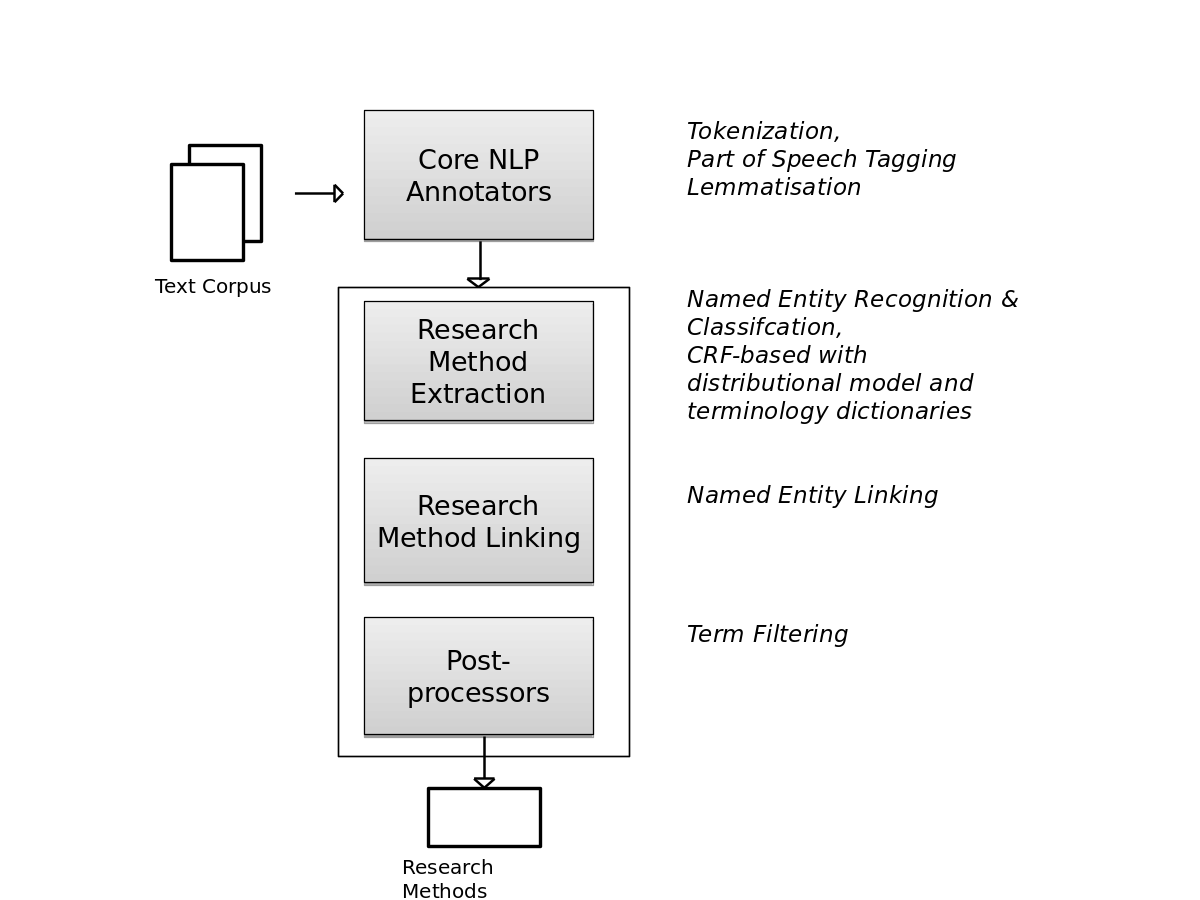
\includegraphics[width=0.47\textwidth]{figures/research-methods/pipeline.png}
    \caption{Overview of the entity extraction pipeline}
\end{figure}

\paragraph{Distributed Semantic Models}%\ \\[1pt]
\label{subsec:dist-model}
For domain adaptation, we integrate further background knowledge. We use vector embeddings  of words trained on additional corpora and which serve as input features to the CRF model. Semantic representations of words are a successful extension of common features, resulting in higher NER performance~\cite{Turian} and can be trained offline.


In this work, the word vectors were learned  from the scientific ACL ARC\footnote{\url{https://acl-arc.comp.nus.edu.sg/}} using Gensim with the skip gram model (cf. \cite{mikolov2013distributed}) 
and a pre-clustering algorithm\footnote{
Word embeddings are trained with a skip gram model using embedding size equal to 100, word window equal to 5, minimal occurrences of a word to be considered 10. Word embeddings are clustered using agglomerative clustering with a number of clusters set to {500,600,700} Ward linkage with euclidean distance is used to minimize the variance within the clusters.}. A summary of the size of the unlabeled  English data used for training word embeddings can be found in Table~\ref{tab:UnlabeledData}.

\begin{table}
\center
\small
  \caption{English data used for Training Word Embeddings}
  \label{tab:UnlabeledData}
  \begin{tabular}{lll}
    \toprule
    Corpus & Articles &  Documents/Tokens  \\
    \midrule
   ACL Corpus
    %ACL Anthology Reference Corpus
    &  22,878  &  806,791/2.5 GB \\ 
  \bottomrule
\end{tabular}
\end{table}

\paragraph{Features}%\ \\[1pt]
The  features incorporated into the linear chain CRF are shown in the Table~\ref{tab:features}. The features depend mainly on the observations  and  on  pairs  of  adjacent  labels, using a log-linear  combination. However, since simple token level training of CRFs leads to poor performance, more effective text features such as word shape, orthographic, gazetteer, Part-Of-Speech (POS) tags, along with word clustering (see Section~\ref{subsec:dist-model}) have been used.
%
\begin{table}
\small
  \caption{Features used for NER}
  \label{tab:features}
  \center
  \begin{tabular}{lc}
    \toprule
  \textbf{Type} &  \textbf{Features} \\
    \midrule
\textbf{Token unigrams} 	   &    $w_{i-2}$, $w_{i-1}$, $w_{i}$, $w_{i+1}$, $w_{i+2}$, ... \\

\textbf{POS unigrams} 	   &    $p_{i}$, $p_{i-1}$, $p_{i-2}$ \\

\textbf{Shapes}	   &    shape and capitalization \\
    \midrule
\textbf{NE-Tag}	   &    $t_{i-1}$, $t_{i-2}$ \\
      \midrule
\textbf{WordPair}	 &   
($p_{i}$, $w_{i}$, $c_{i}$) \\

\textbf{WordTag}	 &   
($w_{i}$, $c_{i}$) \\

    \midrule
\textbf{Gazetteer}	   &    SAGE gazetteer \\
    \midrule
    \textbf{Distributional Model}	   &    ACL Anthology model \\
      \bottomrule
   \end{tabular}
\end{table}

\paragraph{Knowledge Resources}%\ 
We use the SAGE thesaurus which includes well-defined concepts, an explicit taxonomic hierarchy between concepts as well as labels that specify synonyms of the same concept.
A portion of terms is unique to the social science domain (e.\,g.,  `dependent interviewing'), while others are drawn from related disciplines such as statistics (e.\,g., `conditional likelihood ratio test')\footnote{A glossary of statistical terms as provided in \url{https://www.statistics.com/resources/glossary/} has been added as well.}.
However, since the thesaurus is not exhaustive and covers only the top-level concepts related to social science methods, our aim was to extend it by automatically extracting further terms from domain-specific texts, in particular from the Social Science Open Access Repository.
More concretely, we carried out the following steps to extend SAGE as an off-line step. For step 2 and 3, candidate terms have been extracted by our pipeline for the entire SSOAR corpus. 
\begin{enumerate}
\item Assignment of semantic types to concepts (manual) 
\item Extracting terms variants such as abbreviations, synonyms, related terms from SSOAR (semi-automatic)
\item Computation of Term and Document Frequency Scores for SSOAR (automatic)
\end{enumerate}

\paragraph{Extracting term variants such as abbreviations, synonyms, and related terms}%\ \\[1pt]
26.082 candidate terms have been recognized and classified by our pipeline and manually inspected to  
a) find synonyms and related words that could be linked to SAGE, and
b) build a post-filter for incorrectly classified terms.  
Moreover, abbreviations have been extracted using the algorithm of Schwartz and Hearst
\cite{SchwartzH03}.
This way, a Named Entity gazetteer could be built and will be used at run-time. It comprises 1,111 terms from SAGE and 447 terms from the Statistics glossary as well as 54 previously unseen terms detected by the model-based classifier. 




\paragraph{Computation of Term and Document Frequency Scores}%\ \\[1pt]
Term frequency statistics have been calculated off-line for the entire SSOAR corpus.
The term frequency at corpus level will be used at run time to determine the term relevance at the document level by calculating the TF-IDF scores. The most relevant terms from SAGE are listed in Table~\ref{tab:SAGET}.
\begin{table}
\center
\small
  \caption{Most relevant terms from SAGE by Semantic Type}
\begin{tabular}{lll}
  \label{tab:SAGET}
  \textbf{SAGE Term} & \textbf{TF-IDF Score}  & \textbf{Semantic Class}   \\ \hline  
Fuzzy logic	  &	591,29  &		Research Method  \\
arts-based research	 &	547,21  &		Research Method \\
cognitive interviewing  &		521,13  &		Research Method \\  
QCA	 &	463,13  &		Research Method   \\ 
oral history	 &	399,68  &		Research Method \\ \hline  
market research  &		345,37  &		Research Field \\
life events  &		186,61  &		Research Field \\ \hline 
Realism  &		314,34  &		Research Theory \\
Marxism  &		206,77  &		Research Theory \\ \hline  
ATLAS.ti  &		544,51  &		Research Tool\\
GIS	 &	486,01  &		Research Tool\\
SPSS	  &	136,52  &		Research Tool \\ \hline  
  
\end{tabular}
\end{table}


\paragraph{Definition of a Relevance Score}%\ \\[1pt]
\label{para:relscore}
Relevance of terminology is often assessed using the notion of 
\textit{unithood}, i.e. `the degree of strength or stability of syntagmatic combinations of collections', and 
\textit{termhood}, i.e. `the degree that a linguistic unit is related to domain-specific concepts' \cite{kageura1996methods}.
Regarding \textit{unithood}, the NER model implicitly contains heuristics about legal POS tag sequences for candidate terms, 
consisting of at least one noun (NN), preceeded or followed by modifiers such as adjectives (JJ), participles (VB*) or cardinal numbers (CD), complemented by wordshape features.

In order to find out if the candidate term also fulfills the \textit{termhood} requirement, domain-specific term frequency statistics have been computed on the SSOAR repository, and set in contrast to general domain vocabulary terms. 
%\footnote{based on COCA, i.e. a large, balanced Corpus of Contemporary American English, using \textit{spoken, fiction, popular magazines and newspapers} rather than \textit{academic journals}, cf. \url{https://corpus.byu.edu/coca/} with frequency infos at \url{https://www.wordfrequency.info}}. 
It has to be noted  that only a small portion of the social science terms is actually unique to the domain (e.g.,  `dependent interviewing'), while others might be drawn from related disciplines such as statistics (e.g., `conditional likelihood ratio test').


%COMMENT (AZ) Since there is no gold standard it is difficult to report any reliable results! 
\paragraph{Preliminary Results}%\ \\[1pt]
Our method has been tested on 100 fulltext papers from SSOAR and 10 documents from the Rich Context Competition (RCC), all randomly selected from hold out corpora.
In our experiments on SSOAR Social Science publications, we compared results to the given metadata information.
The main finding was that while most entities from the SAGE thesaurus could be extracted and linked reliably (e.g., 'Paired t-test'), they could not be easily mapped to the SSOAR metadata terms, which consist of only a few abstract classes (e.g., 'quantitative analysis'). Furthermore, our tool was tested by the RCC organizer, were the judges reviewed 10 random publications and generated qualitative scores for each document.  %COMMENT (AZ) Yes. We were the winning team on this task. But what results to put here?

%COMMENT (AZ) Please double check 
%\subsubsection{Conclusion and Future Work}
%\label{subsec:ner-conclusion}
%A white paper describing our methods and approach will be published in a refereed special issue of the competition. 
%We plan to carry out a more detailed evaluation on fulltext scholarly publications and assess the impact of different features used in the ML model, including  background resources such as embeddings and dictionaries. 

    
\subsection{Research Field Classification}
\label{sec:field_classification}
\subsubsection{Task Description}
The goal of this task is to identify the research fields covered in the social science publications.
In general, two approaches could be applied to this task.
One is the extraction of relevant terms of the publications.
It means that this task could be seen as a keyword extraction task and the detected terms considered as descriptive terms regarding the research field.
The second approach is to learn to classify publications research fields with the use of annotated data in a superviesed manner.
The benifit of the second approach is that the classification scheme to describe the research field can be defined experts of the domain.
The disadvantage of supervised trained classifiers for this task is the lack of applicable training data.
Furthermore, it must be ensured that the training data is comparable to the texts the research field classifier should be applied on.

%% * Formal definition
\paragraph{Formal problem definition}
Let $P$ denote a set of Publications of size $n$, $A$ a set of corresponding abstracts of the same size and $L$ a set of $k$ defined class labels describing research fields.
The task of research field classification is to select for each publication $p_i\in{P}$ based on the information contained in the corresponding abstract $a_i\in{A}$ a set of labels $C_i = \varnothing \cap \{c_1\dots c_n|c_n \in L\}$ of $n$ labels.
The number of $n$ denotes the number of labels from $L$ describing the research field of $a_i$ and can vary for each publication $p_i$.
If there is no label $l_k$ representing the information given by the abstract $a_i$ the set of class labels is the empty set $\varnothing$.


%\subsubsection{Challenges}
%% * Decision for Supervised
%%  * No Gold standard given
%%  * Known Corpus from similar domain
%%  * benefits of SSOAR corpus
%%  * Why is it good
%%  * Because of courpus we decided to go for a supervied method

\subsubsection{Our approach - Overview}
%% External data (SSOAR
%% * Supervised
%% * Multi label classification
Since we didn't receive any gold standard for this task during the competition we decided to make use of external resources.
We decided to use an external labeled dataset to train a text classifier which is able to predict for a given abstract of a publication one or more research field label.

The publications given througout the competition belongs to the domain of social sciences we considered metadata from a open access repository for the social sciences called SSOAR.
The advantages are twofold.
On the ond hand, we could rely on professional annotations in a given classification scheme covering the social sciences and related areas.
On the other hand the source is openly available.\footnote{A script to download the metadata of SSOAR can be found in github/research-field-classifier}

%% * Classification schmeme Classoz (Why it seems usefull)
The annotated data of SSOAR contains four different annotation schemes for research field related information. By reviewing these schemes, We decided to use the Classification Social Science (classoz) annotation scheme. The number of classes in each schema, coverage of each classification, and the distribution of data in each schema affected our decision. 
An exhausitve description of the used data can be found in \ref{section:external_data_sources}.

%% * data pre pro
\paragraph{Pre-processing and model architecture}
%%  * selected fields and language
%%  * titles are often german
SSOAR is a multilingual repository.
Also the available abstracts can vary in language which can differ to the language of the publication.
We selected all English abstract with valid classification as our dataset.
Mainly because of the language of the RCC corpus.
But it has to be noted, that the multilingual SSOAR-abstract-corpus has a skewed distribution of languages with English and German as the main languages.
We count 22,453 English abstracts with valid classification after filtering.
%%  * skipped label
Due to the unequal distribution of labels in the dataset, we need to guaranty enough training data for each label.
We selected only labels with frequency over 300 for training the model, which results in a total of 44 out of 154 classification labels representing research fields.
%%  * Train test split
For creating train and test set, 22,453 SSOAR publications with their assigned labels were split randomly.
We used a train/validation/test split of 70/10/20.
%%* Our model
We decided to train a text classifier based on the fasttext framework~\cite{joulin2017bag}.
The arguments to use this model was the speed in comparison to a more complex neural net archiecture and the still comparable to state of the art performance (e.g.\cite{wang2018joint}).
%%  General used Fasttext parameter
The model is trained with learning rate 1.0 for 150 epochs.
Also, the negative sampling parameter is set to 25.


\subsubsection{Evaluation}
%% metrics
%%  preci recal f1 micro
%%  ...
%% Parameter Selection
%%  k and threshold
%%  * reduced number of labels?
In this experiment, only the top 3 labels with the highest probabilities were considered for the evaluations.
Figure~\ref{fig:fields_precision_recall} shows the performance of the model regarding various evaluation metrics for different thresholds.
A label is assigned to a publication if the model outputs a probability for the label above the defined threshold.
In multi-label classification, this allows us to evaluate our model from different perspectives. 
As it is illustrated in figure~\ref{fig:fields_precision_recall}, the point that the micro-precision curve and micro recall meet is at the threshold of 0.1.
%% final results
We can see the point as the highest point of micro f1-measure. By increasing the threshold from this point, the micro-precision score is increasing, but the micro recall is falling. By Decreasing threshold, these trends are opposite.  Also, the default threshold doesn't look promising. In spite of micro-precision about 0.7, we have a problem with the very high number of items without any prediction. 
%%  comparison to baseline (SVM?)

%%\subsubsection{Discussion}
%%  What do the results show
%%    For how many samples of the test set do we have prediction
%%    How well is the classifier performing on given classes
%%    Performance on different data can not be measure
%%      results from rcc judges are promissing
%%    Lack of generelizability (domain)



%The x-a  the change of  metrics over different probability thresholds for generating the result.
\begin{comment}

This graph shows the change of different evaluation metrics over different probability thresholds for generating the result. 
The threshold defines the minimum probability of a label which is leading to an assignment.

Orderly, micro precision and micro recall values are 0.5 for threshold 0.1
For this threshold, the model generates a prediction for all items and about half of the items have at least one correct prediction. 
All these metrics remain the same till threshold 0.2. Till threshold 0.6, we can see a dramatic increase in the micro precision and the number of items without any correct prediction. Both of these metrics pass 0.8. On the other hand, micro recall falls to the below of 0.2. In this case, selecting threshold seems hard task, since the conflict point of precision and recall is a threshold about 0.25 but both of these metrics at the point are not more than 0.3 and also we have more than 0.4 items with completely wrong predictions. Also, the default threshold doesn't look promising. In spite of micro precision about 0.7, we have a problem with the very high number of items without any prediction.
\end{comment}

\begin{figure}[t]
\centering
%\subfloat[Random Forest Evaluation]{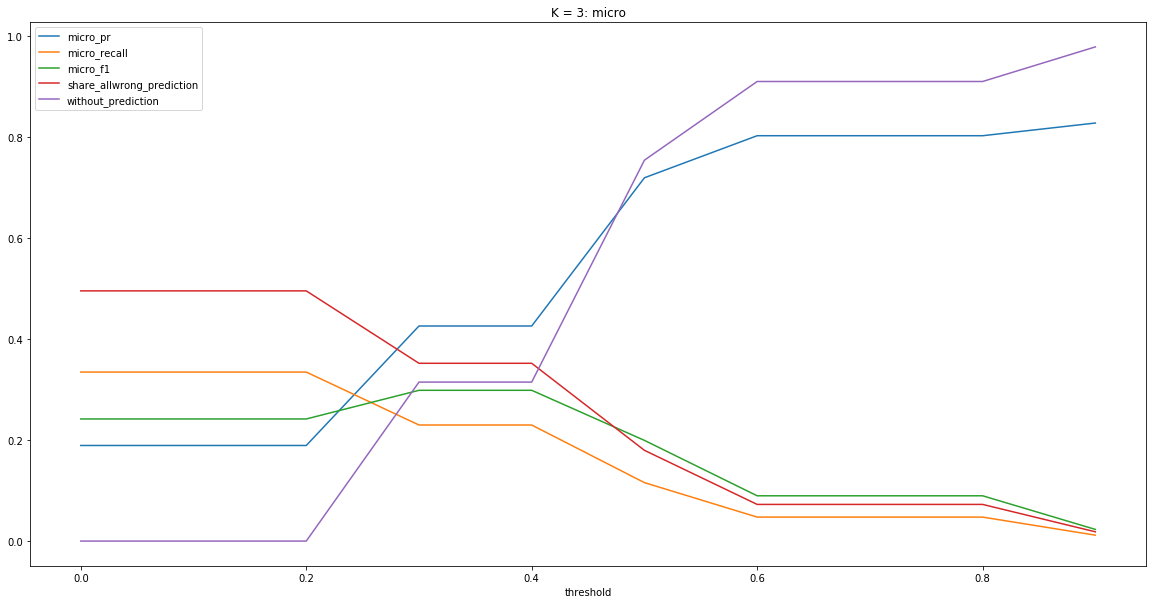
\includegraphics[width=0.49\textwidth]{figures/research-fields/random-forest-evaluation.png}\label{fig:rf}}
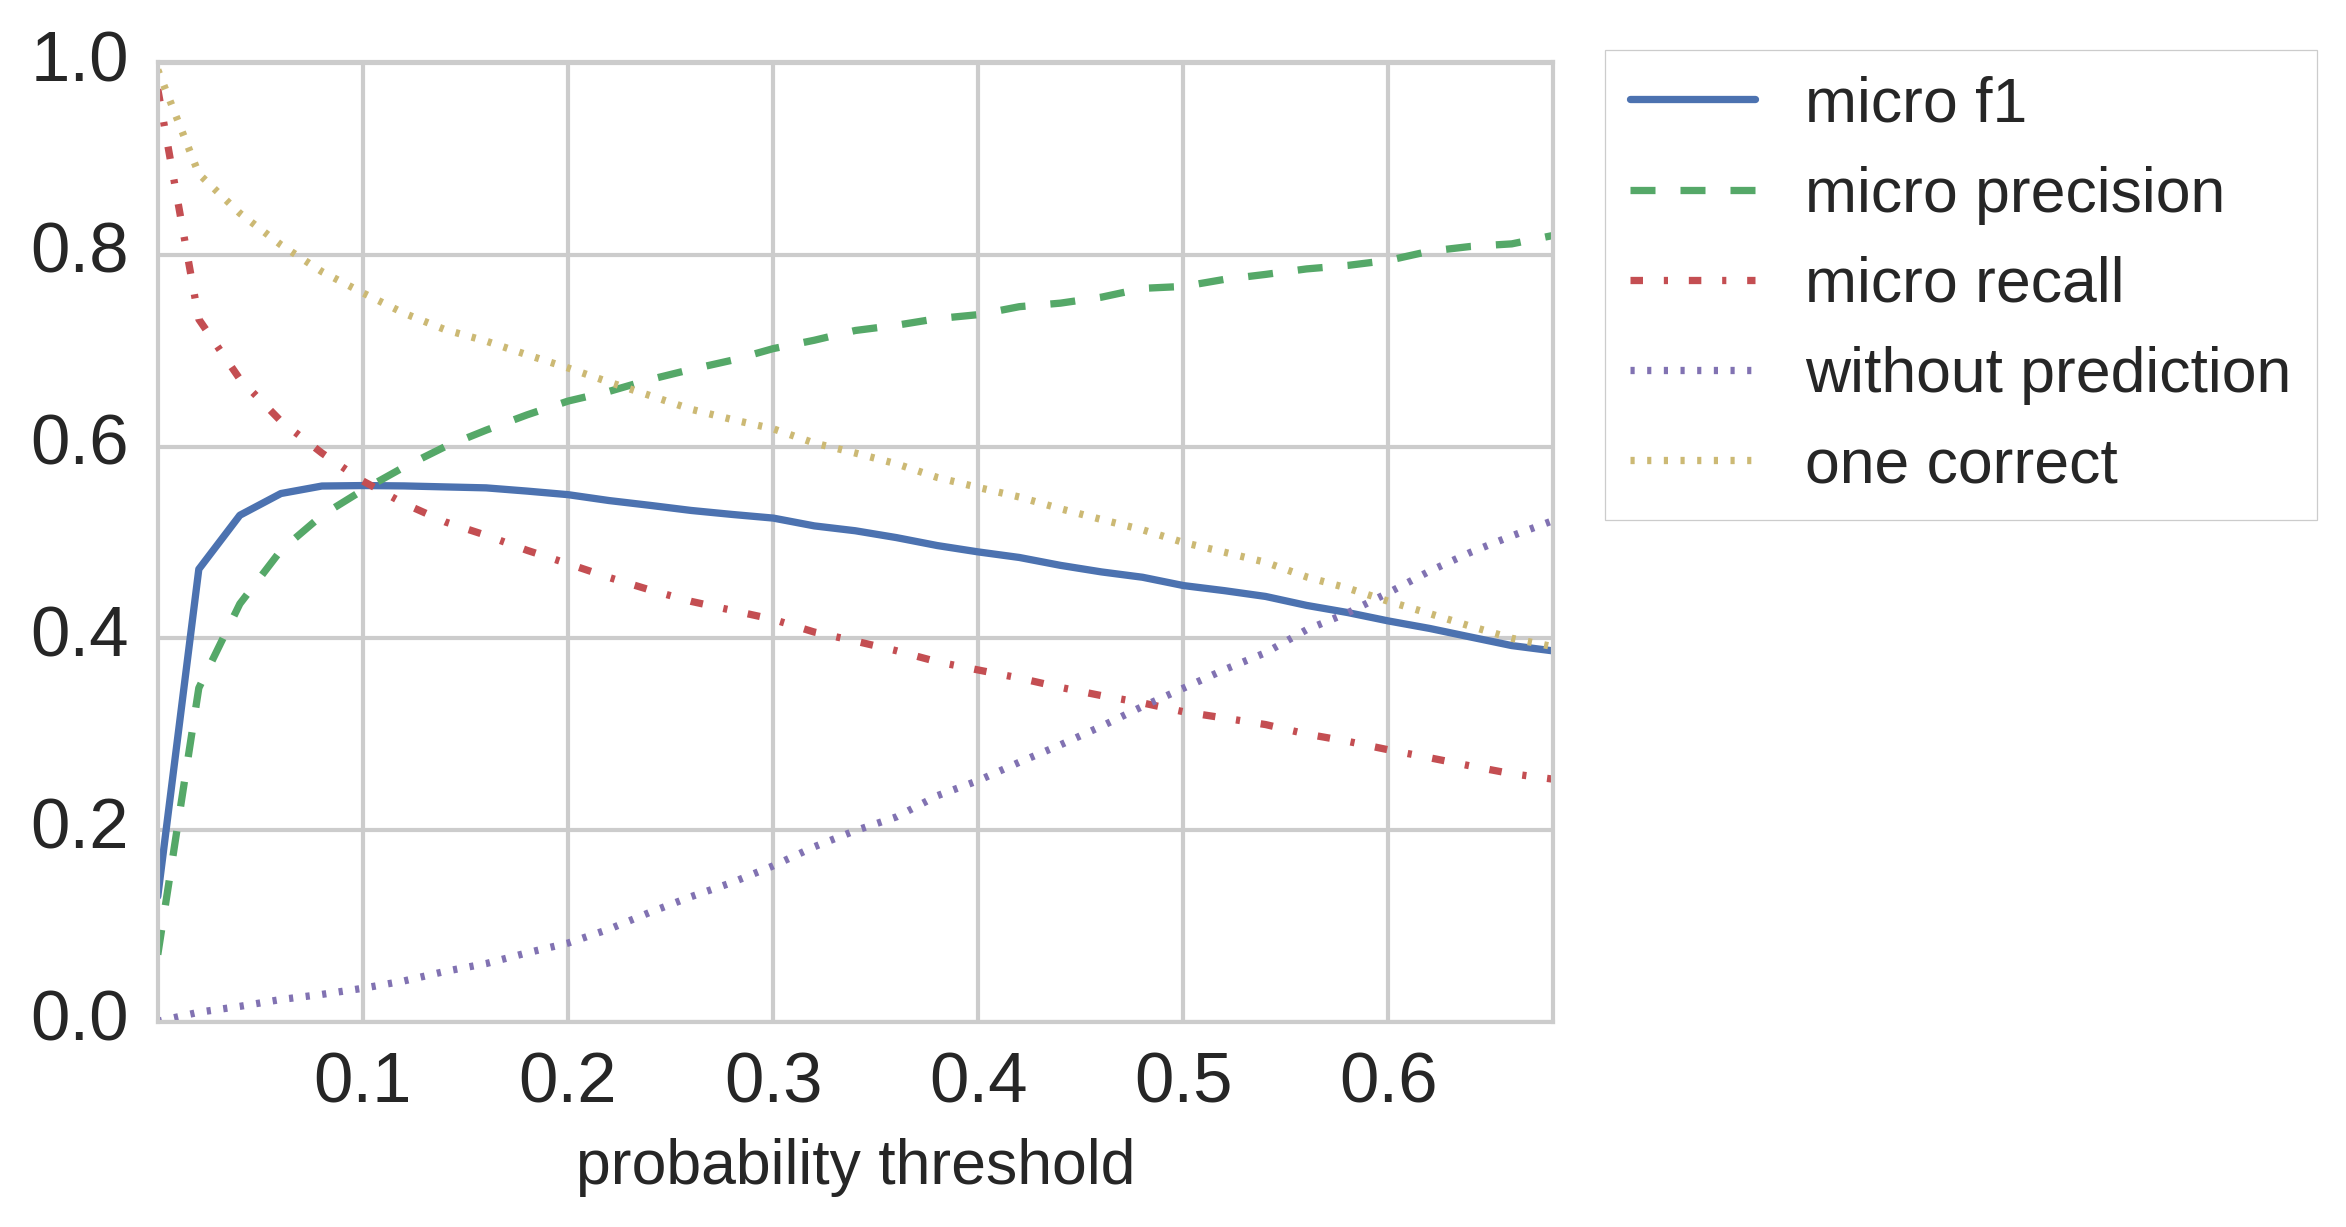
\includegraphics[width=.49\textwidth]{figures/research-fields/fields-precision-recall.png}
%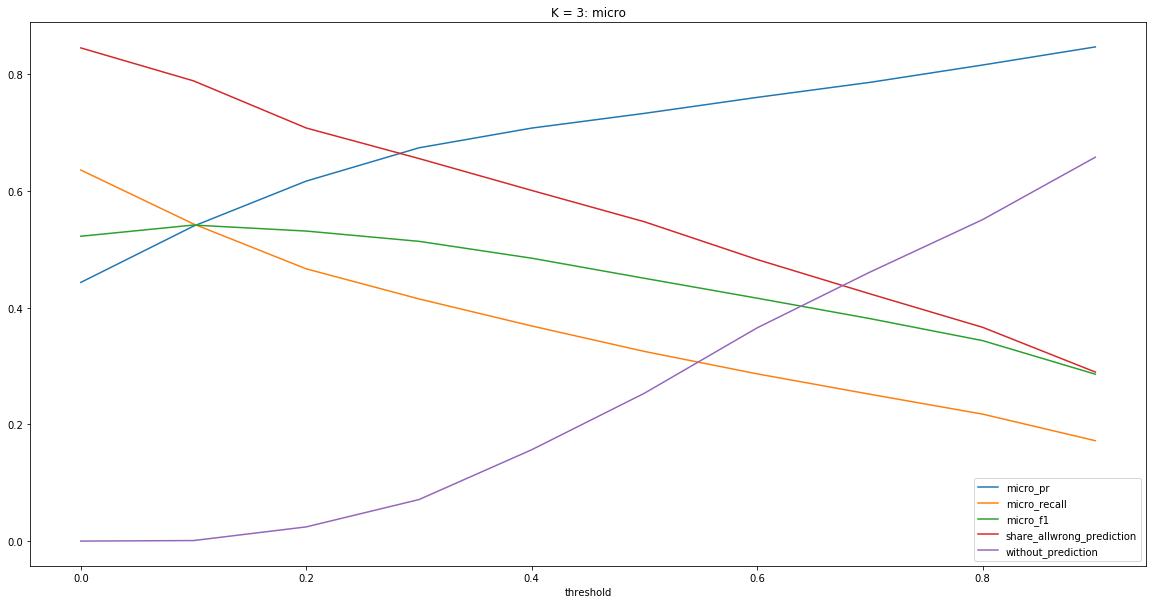
\includegraphics[width=.49\textwidth]{figures/research-fields/fast-text-evaluation.png}
%\vspace{-1em}
    \caption{Metrics for different selected probability thresholds (validation set)}
\label{fig:fields_precision_recall}
\end{figure}


\begin{table}[b]
\center
\small
    \caption{Evaluation results on test set (Fasttext model)}
  \label{tab:eval_research_field}
  \begin{tabular}{ll}
  \toprule
      Metric & Value \\
  \midrule
      Micro F1:          & 0.529 \\
      Micro Precisison:  & 0.499 \\
      Micro Recall: 	 & 0.564 \\
  \bottomrule
\end{tabular}
\end{table}

%The trends of micro f1, micro recall, and publications with just wrong predictions are falling smoothly, but the trend of micro precision and number of publications without any prediction are rising gradually. 
%The Micro precision still is higher than 0.7 for threshold 0.4. Also, the number of items without prediction is lower in threshold 0.4 than threshold 0.5 (the difference is about 0.1).

% We also experiment with random forest 



%purple curve (without_prediciton) 
%The measure without_prediction describes the share of publications without any prediction at all.
%E.g. if we only accept predicted labels with a model certainty of 60\%, 40\% of the publication have no predictions. 

%red curve (share_allwrong_prediction)
%The red curve describes the share of documents in the test set, which contain only wrong predictions for each threshold.
%This means when a threshold of 20\% certainty is selected 70\% of the publications have only wrong predictions. But if a threshold of 80\% certainty is selected only 40\% of the publications have only wrong predictions. 

    \subsection{Discussion}
\label{sec:discussion}
% Structure suggestions from Julia Lane

%\subsubsection{what-worked-what-not}
%\subsubsection{summary-of-results-and-caveats}
%\subsubsection{lessons-learned-and-what-would-you-do-differently}
%\subsubsection{what-comes-next}

%In this section we discuss our approaches for each of the three tasks.

%The paper presents/has presented several solutions to
\subsubsection{Dataset Extraction}
For the dataset extraction task the proposed method are only tested on social science related data.
The performance measures we have introduced are based on a hold out data set of our automatically created dataset.
Especially the recall could be biased.
This is because we only label known data set.
The results of the second phase presented during the RCC workshop\footnote{
    Agenda of the Workshop: 
    \url{https://coleridgeinitiative.org/richcontextcompetition/workshopagenda}.
    The results of the finalists are presented here: 
    \url{https://youtu.be/PE3nFrEkwoU?t=9865}.
}
are showing good performance of our approach in comparison to the other finalist teams with the highest precision 52.2\% (second: 47.0\%) and second in recall (ours: 20.5, best: 34.8\%).
%, 39.6\% and 33.3\%)
This lead to the second best performing system for this task in respect of f1 measure (29.5\%, 40.0\% first place).
The results on the manually created hold out set pointing out, that our system performs better in respect to precision in comparison to the other finalist teams.
%This could be affected by the decision to annotate only full dataset titles during the automatic annotation process.
%In comparison to the usage of the ground truth term set there are nearly no abbreviation. 
The social science focused corpus of research publications and dataset metadata lead us to suppose, that our trained model is working bad on different domains of science.
Especially the focus on survey data and the reflection in dataset names (e.g. Current Population Survey) could have biased the model to detect the survey as a specific type of research datasets better than other subtypes like e.g. text corpora in the NLP community.
In general our apporach to use a weakly labled corpus created using a list of datast names could be applied in other research domains.
The needed roussources are a set of full text publications and a sufficiently large list of dataset names for this domain.
\begin{comment}
* limitations\
**    Performance is difficult to measure\\
**    Ground truth needed to have a good measure\\
**    During development a ground truth holdout set would have prevented the feeling to fish in troubled waters.\\
%One of the biggest problems of the dataset extraction task was to handle abbreaviations.
\end{comment}

\subsubsection{Research method extraction}
The extraction of research methods from full text publications we consider as the most challenging task.
This is because, the sample vocabulary given by the competition covers a large thematic area, from dataset, over mathematical models to qualitative methods.
The task itself was defined as the identification of research methods associated to the publication.
On the one hand we were confronted with a lack of training data in the competition.
On the other hand, in contrast to the task of research field classification, we were not able to identify external corpora which could be applied on this task.
We combined models from another research domain with a manually currated extension of known research method terms.
The qualitative reviews during the two phases of the competiton attested that this approach works.
A valid quantitative evaluation is prevented by the lack of ground truth data.

\subsubsection{Research field classification}
Our supervised machine learning approach to handle the research field classification task performs well on the dataset created from social science publication metadata.
A micro f1 measure of above 55\% seems to be a good result for a dataset with 44~labels and a mean number of keywords of three terms per publication.
As one example of multilabel classification with a comparable size of labels we would like to mention the classification of texts in the domain of medicine presented in \cite{wang2018joint}.
The models tested by the authors on the task of multilabel prediction from 50 different labels leads to micro f1 values between 53\% and 62\%.\\
% Compare https://arxiv.org/pdf/1805.04174.pdf (5.3 Applications to Clinical Text) There micro f1 is above 60\% :-(
The analysis of the performance of our model does not enable us to determine the performance on other research domains than the social sciences.
Even if the used classification scheme covers neighbour disciplines like medicine, the numbers of samples of the training data covering other research fields than the social science is less.
If one considers this fact, it can be assumed that the performance for corpora of other disciplines is lower.
A benefit of our approach is the usage of abstracts as input to classify the research publications.
This make the approach usefull even if there are no full text of publications are available.
On the other hand, the use of Cermine to extract information from publications available as PDF files enables us to automatically extract abstracts.
With the help of this we are able to classify publications, even if abstracts not present in the publications metadata.

%For each method, brief summary of:
%\begin{itemize}
%\item results / performance
%\item applicability / generalisability
%\item limitations and challenges (eg lack of large-scale GT, corpus-specific training etc etc)
%\end{itemize}


    \subsection{Conclusion}
\label{sec:conclusion}
This chapter has provided an overview on our solutions submitted to the Rich Context Competition 2018. Aimed at improving search, discovery and interpretability of scholarly resources, we are addressing three distinct tasks all aimed at extracting structured information about research resources from scientitifc publications, namely the extraction of dataset mentions, the extraction of mentions of research methods and the classification of research fields. 

In order to address all aforementioned challenges, our pipelines make use of a range of preprocessing techniques together with state-of-the-art NLP methods as well as supervised machine learning approaches tailored towards the specific nature of scholarly publications as well as the dedicated tasks. In addition, background datasets have been used to facilitate supervision of methods at larger scale.

Our results indicate both significant opportunities for automating the aforementioned three tasks but also their challenging nature, in particular given the lack of publicly available gold standards for training and testing. Aggregating and publishing such data has been identified as important activity for future work, and is a prerequisite for significantly advancing state-of-the-art methods.

%TODO Stefan will expand this with more comprehensive discussion/future directions section at some point.

    %\section{Technical Documentation}
\label{sec:techdoc}
%(Documentation on how to install, train, configure, and run the model program)
The project contains the following modules listed in the order in which they are excecuted.

%=====================================================================================
%=====================================================================================
\subsection{Pre-processing}
%=====================================================================================
\subsubsection{PDF Text Extraction}
\textbf{Module name : }

Cermine_NlmJat_extractor\\
\textbf{Function: }

Converts each PDF files of a given folder to JATS XML Format. Each input PDF File is transformed to one XML File.\\
\textbf{Bash function call: }
\begin{lstlisting}
java -jar target/cermineXMLextraction-1.0.0-jar-with-dependencies.jar
\end{lstlisting}
\textbf{Parameter (2): }
\begin{lstlisting}
-s <source folder>\
-t <target folder>
\end{lstlisting}
\textbf{Returns: }

XML Files in JATS XML Format.\\
\textbf{Build: }

This is a Java program using Maven build tool.\\
\textbf{build call: }

mvn install

%=====================================================================================
\subsubsection{Extraction of text from JATS XML}
\textbf{Module name : }

preprocess-rcc-data\\
\textbf{Function: }

Transform text from JATX XML Format into a JSON File containing a list of textfields with essential metadata for each JATS XML file of a given folder.\\
\textbf{Bash function call: }
\begin{lstlisting}
`python3  ./jats_text_extractor.py `
\end{lstlisting}
\textbf{Parameter (4): }
\begin{lstlisting}
<source folder>
<target folder>
<limiting number of files to transform (-1: all)> 
<number of cores to use for multiprocessing (-1: all)>
\end{lstlisting}
\textbf{Returns: }

A JSON File for each given XML File in the source folder

%=====================================================================================
\subsubsection{Metadata Extraction}
\textbf{Module name : }

preprocess-rcc-data\\
\textbf{Function: }

Extracts structured metadata and references from all JATS XML files in a given folder into two Files.
One containing the metadata from all Publications in JATS XML files and one containing all references from the JATS XML Files.
The target file format is JSON.\\
\textbf{Bash function call: }
\begin{lstlisting}
python3  ./jats_metadata_extractor.py
\end{lstlisting}
\textbf{Parameter (3): }
\begin{lstlisting}
<source folder>
<target filename for metadata>
<target filename for references>
\end{lstlisting}
\textbf{Returns: }

Two JSON files containing metadata and references from all XML Files

%=====================================================================================
%=====================================================================================
\subsection{Dataset Mentions}
%=====================================================================================
\subsubsection{Dataset Mention Extraction}
\textbf{Module: }

dataset-mention-extraction\\
\textbf{Function:}

Extract dataset mentions from all JSON Files from a given folder with a given spacy model.\\
\textbf{Bash function call: }
\begin{lstlisting}
python3  ./predict_mentions.py
\end{lstlisting}
\textbf{Parameter (4): }
\begin{lstlisting}
<source folder>
<name of spacy model folder>
<target filename rcc-output>
<target filename internal format>
\end{lstlisting}
\textbf{Returns: }

Two JSON files containing the found dataset mentions in all given JSON Files.
One in RCC defined output.
One in Internal format including the senctence the dataset mention occures.\\
\textbf{Train: }

For training we submit a jupyter notebook with all needed code.
\emph{Train_spacy_ner_prod.ipynb}\\
\textbf{Build (For training only): }

Install english spacy language model.
This can be done with `python -m spacy download en`.

\begin{comment}
\textfg{}
For evaluation we first predict with the predictor which is used in production `predict_mentions.py`. We run this script on the test data and the result is a new field in paragraph data called `predicted_standoff`.
During evaluation with `evaluate.py` this filed is compared to the `standoff` field. The only parameter `evaluate.py` needs is the filename of the test data and the filename where the results should be saved in json format.
\end{comment}


%=====================================================================================
\subsubsection{Dataset Linking (only Phase 1)}
\textbf{Module: }

dataset-prediction\\
\textbf{Function: }

Links dataset mentions given a JSON file in internal format to datasets listed in a given JSON File.\\
\textbf{Bash function call:}
\begin{lstlisting}
python3  ./retrieve.py
\end{lstlisting}
\textbf{Parameter (3): }
\begin{lstlisting}
<JSON filename of extracted mentions>
<JSON filename of dataset list to match>
<output filename for dataset citations>
\end{lstlisting}
\textbf{Returns: }

JSON file in the format defined by the competition containing information about links between publications and datasets.

%=====================================================================================
%=====================================================================================
\subsection{Research Method Extraction}
\textbf{Module name : }

research-method-extractor\\
\textbf{Function: }

Extracts research method terms from JSON files with text information from publications.\\
\textbf{Bash function call: }
\begin{lstlisting}
java -jar target/gesisents-0.1-jar-with-dependencies.jar
\end{lstlisting}
\textbf{Parameter (3): }
\begin{lstlisting}
<source folder>
<target file name>
<Limit to reduce the number of processed files (-1:all)>
\end{lstlisting}
\textbf{Returns: }

A JSON file in the format defined by the competition containing information about publications and research methods.
\textbf{Build: }

This is a Java program using Maven build tool.\\
\textbf{build call: }

mvn install


%=====================================================================================
%=====================================================================================
\subsection{Research Field Classifier}
\textbf{Module name : }

research-field-detector\\
\textbf{Function: }

Classifies given abstracts with classoz Labels\\
\textbf{Bash function call: }
\begin{lstlisting}
python3  ./fasttext_predictor.py
\end{lstlisting}
\textbf{Parameter (4): }
\begin{lstlisting}
<filename of JSON file with abstracts>
<filename of fasttext model>
<filename of label dictionary in JSON>
<target filename labels in >
\end{lstlisting}
\textbf{Returns: }

A JSON file in the format defined by the competition containing information about publications and research fields.

\begin{comment}
#### 1. The classifier of FastText library (word embedding),
For training the fastText algorithm, the following code should be run:
```sh
python train_fastext_model.py
```
 In this code, for training the classifier, negative sampling 25 , epoch 150 , and ngram 2 are used as parameters. Also for applying the trained model on some test samples, the following script should be used:
 ```sh
python fasttext_predictor.py data_filename model_filename  label_dict  target
```
#### 2. Random forest algorithm from skilearn library
For training a random forest model, the following command can be used:
 ```sh
python train_sklearn_model.py
```
For training the classifier,  n_estimators=500, and random_state=42 are used as prameters. For applying the trained model on tes# Research Field Detector
t data, the following code should be use:
 ```sh
python sklearn_predictor.py
```
\subsubsection{SSOAR -- Metadata Harvestor}
For this reason a code is implemented to harvest metadata information. Here you can see how to run the harvestor 

code:
```sh
python harvest_ssoar.py
```
\subsubsection*{Evaluation}
For the evaluation, the following file can be used:
```sh
 ./evalouation_part/Evaluation_sklearn.ipynb
```
\end{comment}

    \phantomsection
\subsection{Acknowledgments} 
\addcontentsline{toc}{section}{Acknowledgments}
This work has been partially funded by Deutsche Forschungsgemeinschaft (DFG) under grant number MA 3964/7-1. \\
Wolfgang Otto acknowledges the enabling support provided by the Indo-German Joint Research
Project titled ‘Design of a Sciento-text Computational Framework for Retrieval and
Contextual Recommendations of High-Quality Scholarly Articles’ (Grant No.
DST/INT/FRG/DAAD/P-28/2017) for this work. 
%\phantomsection
\subsection{References} 
\bibliographystyle{unsrt}
\bibliography{bibliography}

\end{document}



% July 2019:
% Tasks: (unfortunately in german)

%    Eine bessere Einleitung  (Siehe Stichpunkte)
%        Anfrage an Stefan laeuft: Wenn du da gesis/wts Einleitung Textbausteine hast würde ich die gerne Einbauen
%    Researchfield Classifier ausführlicher
%        Workshop Nachfrage (Warum auf 44 Klassen beschränkt?) beantworten, bessere Grafik
%        Kann hier Grafiken von Nihal nutzen
%    Discussion Teil (Orientiert an den Anregungen von Julia Lane - Lessons learned ... (Siehe markdown dokument)
%        Beispiel Extraktionen (Datensätze diskutieren)


%% 
%% Review of white paper
%% o   Clear overview of tasks
%% o   Solid presentation of approach
%% o   Major advantage given their local dataset:  Social Science Open Access Repository %% (SSOAR) – but use what you have is a GREAT principle.
%% o   Professional effort!!!  -- Approach, documentation, & justification.
%% o   Problem:  quality of their results, lower than others.

% all
% ------
%•	In both field and dataset classification, what types of errors did you get? Were these the type of errors you would expect or were there strange ones? Are your errors coming from contextual features or from noun phrase features?

%% Todos:
% research methods:
% ----------------
%"I would have liked to have seen a little more information on the shape features"

% research fields:
% ----------------
% "why did you choose 44 fields"
% More about source of classification
% "•	If, instead of abstracts, you train on summarizations, how do you think it will affect your results?"

% datasets:
%•	You may want to consider looking into the area called ‘weak supervision’. Specifically, you mentioned that some of the things that spaCy model was returning looked good, and you could add those in as an additional training data - other terms for that could be ‘co-training’ or ‘bootstrapping’.
% No. weak supervision

% Words about matching (citation?) •	You said that the mentions problem was more interesting to confront than citations - do you have any thoughts on why you performed worse on the citation problem than on the mentions?

